\documentclass[../main.tex]{subfiles}

\begin{document}

\begin{figure}[H]
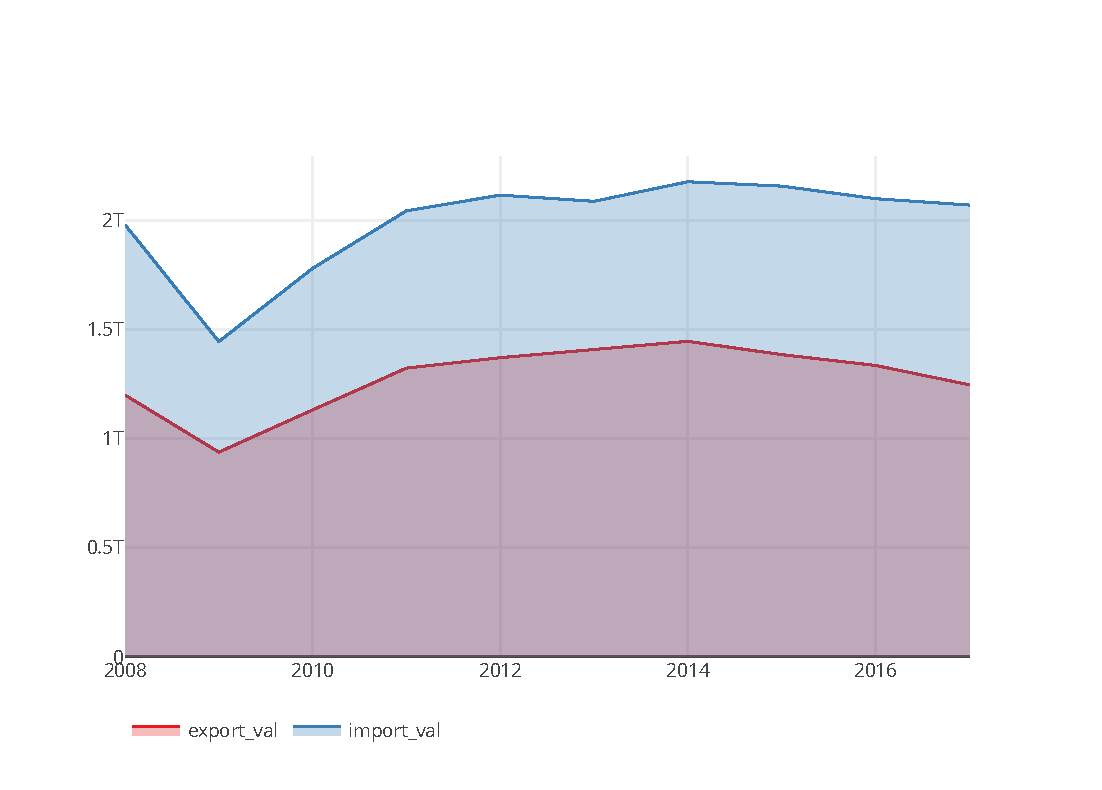
\includegraphics[width=\linewidth]{trade_balance.pdf}
\caption{USA trade balance between 1960 and 2017}
\end{figure}

\subsection{Trade openness}

\begin{figure}[H]
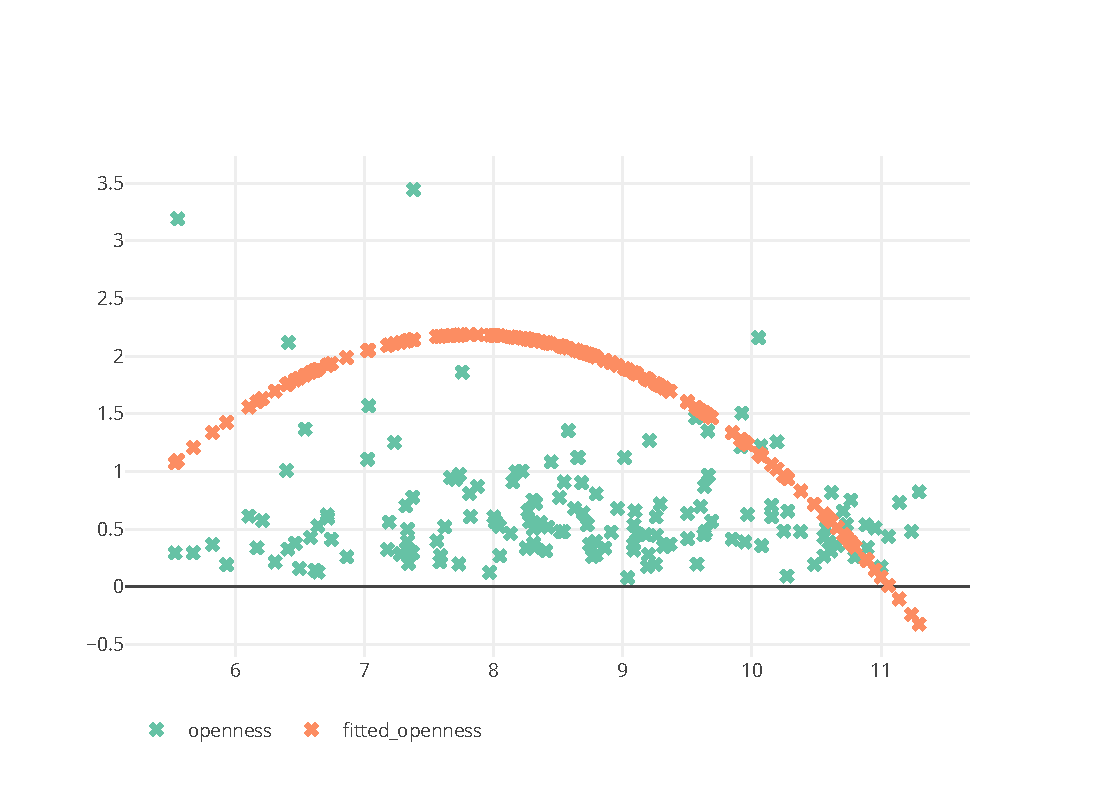
\includegraphics[width=\linewidth]{trade_openness.pdf}
\caption{Quadratic regression of Trade Openness to the $\log$ of GDP per Capita in 2017}
\end{figure}

\comm{Vertical specialization: compare across NAFTA}

\subsection{Trade composition}

\subsubsection{Secotral composition of USA trade}

\comm{perhaps to for exports / imports}

\subsubsection{Intra-industry trade}

\comm{Intra industry trade: see if can apply on NAFTA only}
\comm{Export diversification: Herfindahl index + Hummels and Klenow}

\subsection{Comparative advantage}

\subsubsection{Revealed comparative advantage}

\comm{Across NAFTA}

\subsubsection{Revealed technology content: PRODY and EXPY indexes}

\subsubsection{Regional trade: NAFTA}

\comm{Import matrix}
\comm{regional intensity of trade}
\comm{Trade complementarity: Across NAFTA (matrix)}







\end{document}